% $2^3$ es ejemplo de retículo
% Incluido
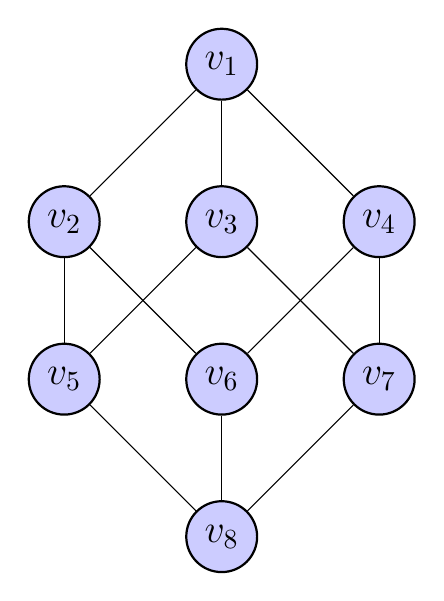
\begin{tikzpicture}[
  scale=2,
  vnode/.style={circle, fill=blue!20, draw=black, thick, minimum size=9mm, inner sep=0pt, font=\Large}
]
  % Vértices
  \node[vnode] (v1) at (1, 3) {$v_1$};
  \node[vnode] (v2) at (0, 2) {$v_2$};
  \node[vnode] (v3) at (1, 2) {$v_3$};
  \node[vnode] (v4) at (2, 2) {$v_4$};
  \node[vnode] (v5) at (0, 1) {$v_5$};
  \node[vnode] (v6) at (1, 1) {$v_6$};
  \node[vnode] (v7) at (2, 1) {$v_7$};
  \node[vnode] (v8) at (1, 0) {$v_8$};

  % Aristas
  \foreach \from/\to in {v1/v2, v1/v3, v1/v4, v2/v5, v2/v6, v3/v5,
                         v3/v7, v4/v6, v4/v7, v5/v8, v6/v8, v7/v8}
    \draw (\from) -- (\to);
\end{tikzpicture}
